\chapter{Многоногий шагающий аппарат с трёхзвенный корпусом}
\label{articulated}

\section{Описание модели трехзвенного робота}

Для описания компьютерной модели, в которой будет исследоваться движение многоногого шагающего аппарата, необходимо задать следующие объекты:

\begin{itemize}
\item система твердых тел из которых состоит робот и объекты моделируемой сцены;
\item наложенные на систему тел связи --- шарниры, которыми соединены между собой части робота;
\item управляющие шарнирные моменты;
\item контактное взаимодействие тел между собой.
\end{itemize}

После ввода перечисленных выше объектов в программный комплекс Универсальный Механизм (УМ), программные средства автоматически выведут уравнения движения системы. Полученные таким образом уравнения можно численно интегрировать набором встроенных методов и наблюдать за состоянием системы в реальном времени при помощи средств визуализации.

\begin{figure}[ht]
  \centering
  \includegraphics[width=0.7\linewidth]{Articulated/robot_2.eps}
  \caption{Шестиногий робот с трехзвенным корпусом}
  \label{articulated:fig:robot}
\end{figure}

Рассмотрим шестиногий робот с трехзвенным корпусом на рисунке \ref{articulated:fig:robot}. Робот состоит из 21 тела --- трехзвенный корпус и шесть ног по три звена в каждой. Кроме того, в систему включаются тела, соответствующеи препятствиям, которые требуется преодолеть. В данном разделе будем рассматривать препятствие в виде высокого уступа, на который робот должен будет залезать при помощи кулоновского трения. На рисунке \ref{articulated:fig:cliff} изображена начальная позиция робота для преодоления препятствия уступ.

Наложенные на систему связи задаются посредством задания обобщенных шарниров в редакторе модели. Данный подход подробно описан в руководстве пользователя \todo{ссылка} и обучающих материалах \todo{ссылка}.


Шарнирные моменты вырабатываются при помощи следящей системы на основе ПИД регулятора \todo{ссылка}. Коэффициенты усиления в регуляторе настраиваются таким образом чтобы шарниры следовали заданному программному значению с необходимой точностью в предположении, что в каждый момент времени доступна точная информация обо всех обобщенных координатах системы. Программные значения формируются в результате работы алгоритмов управления.
При построении движения считаем, что робот взаимодействует с опорными поверхностями только стопами; ноги не должны пересекаться с корпусом и между собой. Стопы не оборудованы присосками и какими-либо дополнительными приспособлениями. На систему действует сила тяжести.

Приступим к детальному описанию перечисленных компонент.

Корпус робота состоит из трех одинаковых звеньев в форме параллелепипеда массы $m$ и cо сторонами $a,b,c$. Каждая из шести ног робота состоит из трех звеньев длины $l_1,l_2,l_3$ и массы $m_1,m_2,m_3$ соответственно.

Для описания шарнирных углов корпуса, введем системы координат $C_ix_iy_iz_i$ связанные со звенями корпуса, где индекс $i$ принимает значения $i = F,M,R$ для переднего, среднего и заднего звена соответственно. Начала $C_i$ систем координат расположены в центрах звеньев, оси $Cx_i$ направлены в продольном направлении корпуса, оси $Cz_i$ -- вдоль строительных вертикалей звеньев, оси $Cy_i$ дополняют соответствующую систему до правой тройки.
Звенья корпуса соединены между собой при помощи одностепенных вращательных шарниров. Все оси вращения шарниров корпуса направлены в поперечном направлении корпуса -- вдоль осей $Oy_i$. Соотношение связывающее системы координат двух соседних звеньев можно записать в виде выражения в однородных координатах:


\todo{матричное выражение}

К каждому сегменту корпуса крепится по две ноги -- правая и левая. Точка крепления ноги и ориентация системы координат ноги относительно системы координат сегмента корпуса задаются при помощи следующего соотношения.


 Точки крепления ног в системе координат $i$-го сегмента:

\todo{выражение}

Кинематика ног является инсектоморфной --- подражает кинематике ног насекомых. В мире насекомых очень много моделей ног -- они зависят от специализации. Но они все имеют общую морфологию -- состоят из одинакового набора сегментов. На рисунке \todo{рисунок} приведены основные виды ног и подписаны названия сегментов.

Рассмотрим кинематику ног. На рисунке \todo{вставить рисунок} изображена кинематическая схема ноги. Шарнирные углы $\alpha,\beta,\gamma$ определяют положение $(x,y,z)$ конца ноги в системе координат связанной с точкой крепления ноги:

\begin{equation}
  \text{формула прямая кинематика}
\end{equation}

По заданному целевому положению конца ноги в системе координат ноги можно однозначно восстановить шарнирные углы, решив задачу обратной кинематики. Решение обратной задачи:

\begin{equation}
  \text{формула обратной задачи}  
\end{equation}

Всего у робота 26 степеней свободы --- по 3 в каждой из ног и 8 степеней свободы у корпуса.

Отношение геометрических величин примем следующим

\begin{equation}
\label{articulated:ratio}
  a:b:c:l_1:l_2:l_3:H = ....
\end{equation}

где $H$ -- высота уступа.

\subsection{Формирование динамической модели робота}
В рамках данного раздела обозначим $q = (q_1, ....q_8)$ -- обобщенные координаты корпуса, $q_i = (...)$ -- обобщенные координаты ног, i = 1....6. q = .... -- набор всех координат.

Уравнения Лагранжа в данном случае имеют структуру [31\todo{ссылка номер 31}]:

\begin{equation}
\text{общий вид уравнений лагранжа для робота}
\end{equation}

где M - матрицы масс, K - векторы сил инерции, Q  - векторы обобщенных сил, связанные с действием сил тяжести и реакций опоры. i=0...6 где 0 соответствует корпусу, а 1,...,6 соответствуют ногам. U - векторы управляющих шарнирных моментов.

Программный комплекс Универсальный Механизм автоматически генерирует все части этих уравнений, кроме векторов U и  частей Q связанных с реакциями опоры. Управляющие моменты U задаются следящими системами, целью работы которых является реализация программных значений шарнирных углов. Предлагаемый в работе алгоритм вырабатывает значения U, обеспечивающие устойчивое выполнение требуемых движений.


\subsection{Параметризация шагового цикла}

Рассмотрим задачу равномерной параметризации траектории при помощи параметра $\lambda(t)$, когда закон изменения величины $\lambda$ должен иметь сглаживания в начале и в конце периода $T$. Так считаем что $\lambda$ принадлежит интервалу [0,1], где 0-- соответствует начальному положению на траектории, а 1 -- конечному положению на траектории.

Что обеспечить горизонтальные касательные в точках 0 и 1 к графику $\lambda(t)$, производная $\dot{\lambda}$ должна иметь форму трапеции \todo{рисунок} рисунок. Наклонные участки -- разгон и торможение в начале и в конце соответственно, горизонтальный отрезок -- участок с постоянной скоростью движения. Параметр $t_a$ задает абсолютное значение длительности периодов разгона и торможения. Параметр $T$ задает длительность периода на котором работает параметризация. На рисунке \todo{рисунок} изображен пример графика для $\dot{\lambda}$ и $\lambda$.

Из постановки задачи имеем:

\begin{equation}
  \label{param:eq_1}
  \int\limits_0^T\dot{\lambda(t)}dt = 1  
\end{equation}

Из уравнения \ref{param:eq_1} получаем:

\begin{equation}
  \label{param:max_lambda}
\begin{alignedat}{1}
  (T - t_a) \cdot \dot{\lambda}_{max} = 1\\
  \end{alignedat}, \text{ где } \dot{\lambda}_{max}  \text{ максимальное значение } \dot{\lambda}(t).
\end{equation}

Найдем закон изменения $\lambda(t)$ на участке разгона. При $0 < t < t_a$ обозначим:

\begin{equation}
\label{param:case_1}
\left\{
  \begin{alignedat}{1}
    &\dot{\lambda}_1(t) = \dfrac{\dot{\lambda}_{max}}{t_a}\cdot t,\\
    &\lambda_1(t) = \int \limits_0^{t}\dot{\lambda}_1(\xi)d\xi = \int\limits_0^{t}\dfrac{\dot{\lambda}_{max}}{t_a}\cdot{\xi}d\xi = \dfrac{\dot{\lambda}_{max}}{t_a}\cdot \dfrac{t^2}{2} = \dfrac{t^2}{2t_a(T-t_{acc
      })}.\\
  \end{alignedat}
\right.
\end{equation}

Далее, на участке равномерного изменения $\lambda(t)$ при $t_a < t < T-t_a$ обозначим:


\begin{equation}
\label{param:case_2}
\left\{
\begin{alignedat}{1}
  &\dot{\lambda}_2(t) = \dfrac{1}{T-t_a}, \\
  &\lambda_2(t) = \lambda_1(t_a) + \int \limits_{t_a}^{t}\dot{\lambda}_2(\xi)d\xi = \lambda_1(t_a) + \int\limits_{t_a}^t\dfrac{d\xi}{T-t_a} = \lambda_1(t_a) + \dfrac{t - t_a}{T-t_a}\\  
\end{alignedat}
\right.
\end{equation}


Для участка торможения  $\lambda(t)$ при $T-t_a < t < T$ обозначим:

\begin{equation}
\label{param:case_3}
\left\{
\begin{alignedat}{1}
  &\dot{\lambda}_3(t) = \dot{\lambda}_{max} \cdot \left(1 - \dfrac{t - (T-t_a)}{t_a}\right)\\
  &\lambda_3(t) = \lambda_2(T-t_a) + \int\limits_{T-t_a}^t \dot{\lambda}_3(\xi)d\xi = \lambda_2(T-t_a) + \dfrac{(t - (T - t_a))(T - t + t_a)}{2t_a(T - t_a)}
\end{alignedat}
\right.
\end{equation}


Нужно учесть произвольный сдвиг по времени $t_s$ для задания времени начала переходного процесса. Это делается заменой $t := t - t_s$ для $\lambda_i(t)$ в выражениях \ref{param:case_1}, \ref{param:case_2} и \ref{param:case_3}. В результате для $\lambda(t)$ при заданных значениях $T, t_acc$ и $t_s$ получаем следующее выражение:

\begin{equation}
\label{param:solution}
\lambda(t) = 
\left\{
\begin{alignedat}{2}
& 0, &t < t_s,\\
&\dfrac{(t-t_s)^2}{2t_a(T-t_a)}, &t_s < t < t_a + t_s,\\
&\dfrac{t - t_s - t_a}{T - t_a} + \lambda_1(t_s + t_a), & t_a + t_s < t < T - t_a + t_s,\\
&\dfrac{(t - t_s - (T - t_a))(T - t - t_s + t_a)}{2t_a(T - t_a)}, & T-t_a + t_s < t < T + t_s,\\
&1, & T+ t_s < t.\\
\end{alignedat}
\right.
\end{equation}

Использование выражения \ref{param:solution} для параметра $\lambda$ в качестве параметра при параметризации траекторий движений позволит выполнять гладкое движение по траектории с разгоном и торможением в начальном и конечном участке траектории соответственно.


\subsection{Нахождение управляющих моментов}
\label{control_torques}
Вычисление управляющих моментов реализуется на основе так называемой следящей системы \todo{ссылка}. В каждый момент времени есть текущее реализовавшееся значение шарнирного угла, известное с высокой точностью. Переходный процесс от текущего положения шарнира к желаемому программному строится в виде стандартного PID-регулятора, где управляющий момент $U$ вычисляется по формуле:

\begin{equation}
  U = k_P (x - x_p) + k_I\int\limits_T (x - x_p)dt + k_D(\dot{x} - \dot{x_p})
\end{equation}

где $x$ и $\dot{x}$ - текущие координата и скорость шарнирного угла, $x_p = x_p(t)$ - желаемое программное положение для шарнира, коэффициенты $k_P, k_I, k_D$ - коэффициенты усиления подлежащие настройке. Коэффициенты усиления подбираются так, чтобы рассогласование фактического и программного значения шарнирного угла уменьшалось экспоненциально быстро и без перерегулирования.

\section{Преодоление препятствия типа уступ. Постановка задачи}

\begin{figure}[ht]
  \centering
  \includegraphics[width = 0.7\linewidth]{Articulated/cliff.eps}
  \caption{Робот и препятствие типа уступ}
  \label{articulated:fig:cliff}
\end{figure}

Препятствие типа "Уступ" состоит из трёх контактных площадок - две горизонтальные площадки и одна вертикальная. Расстояние по вертикали между двумя горизонтальными площадками $h$. В начальный момент времени робот стоит на нижней площадке, на некотором расстоянии от вертикальной стенки. Вертикальная стенка образует прямой угол с горизонтальными площадками. Далее в работе рассматриваем уступ, высота которого равна длине корпуса робота, т.е. размер препятствия является существенным по сравнению с размерами робота.

Практический интерес представляет случай, когда робот преодолевает препятствие только за счет использования сил кулоновского трения. Далее в разделе будем искать условия при которых необходимый коэффициент трения $k$ между ногам робота и опорной поверхностью будет удовлетворять условию:

\begin{equation}
\label{articulated:k_condition}
  0 < k < 1
\end{equation}

Значения, большие единицы, для коэффициента трения означают, что веса аппарата не хватает чтобы создать необходимую силу трения и потребуется использовать специальные зацепные механизмы на концах ног, чтобы обеспечить устойчивость конфигурации.

Считаем, что робот двигается в режиме статической устойчивости и не менее трех ног находятся в контакте с опорной поверхностью. Работ двигается, так называемой, походкой галоп - поочередно переставляя пару симметричных ноги по левому и правому борту. Робот двигается в режиме квази статики, т.е. достаточно медленно.

При залезании на верхнюю горизонтальную площадку прямого уступам можно выделить следующие конфигурации расположения ног робота:

\begin
{enumerate}
  \item все ноги робота опираются на нижнюю горизонтальную площадку
  \item одна пара ног опирается на вертикальную площадку, а другая пара ног опирается на нижнюю горизонтальную площадку
  \item одна пара ног опирается на верхнюю контактную площадку, а другая пара ног опирается на вертикальную площадку
  \item все ноги робота опираются на верхнюю горизонтальную площадку уступа
\end{enumerate}

Исследуем статическую устойчивость робота для каждой конфигурации, когда одна из пар опирается на вертикальную площадку препятствия. 


\subsection{Первая конфигурация}
\label{articulated:case1}

\begin{figure}[ht]
  \centering
  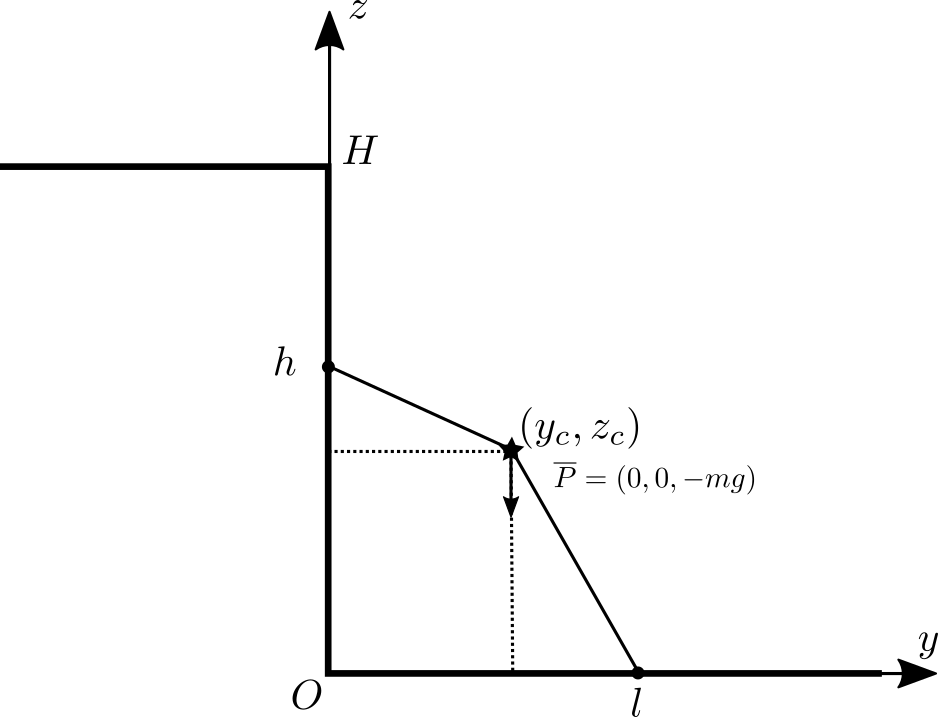
\includegraphics[width = 0.7\linewidth]{Articulated/configuration_1.eps}
  \caption{Робот стоит на нижней горизонтальной площадке и опирается на вертикальную стенку}
  \label{articulated:configuration_1}
\end{figure}


Исследуем на устойчивость конфигурацию, когда одна пара ног робота опирается на вертикальную стенку, а вторая пара ног опирается на нижнюю горизонтальную площадку. Робот будет находится в статическом равновесии, когда сумма всех внешних сил и сумма всех внешних моментов будут равны нулю.

Введём неподвижную систему координат $Oxyz$. Оси системы направлены как показано на рис.(\ref{articulated:configuration_1}) и образуют правую тройку векторов.

Пусть точки опоры ног имеют координаты:

\begin{equation}
  \label{articulated:case_1_step_points}
  \begin{alignedat}{3}
    \overline{r}_1 &= (d, 0, h) , &\overline{r}_2 &= (-d, 0, h) \\
    \overline{r}_3 &= (d, l, 0) , &\overline{r}_4 &= (-d, l, 0) \\
  \end{alignedat},~l>0, h>0, d>0.
\end{equation}


Положение центра масс аппарата задано вектором:


\begin{equation}
\label{articulated:case_1_center_of_gravity}
  \overline{r}_c = (0, y_c, z_c), 0 < y_c < l\\
\end{equation}


На центр масс робота действует сила тяжести:

\begin{equation}
\label{eq:F_c}
  \overline{P} = (0,0,-P)
\end{equation}

В точках контакта ног с опорной поверхностью, на ноги действуют реакции опоры:

\begin{equation}
\label{eq:reactions}
  \overline{R}_i := N_i\cdot\overline{n}_i + F_\tau^i\cdot\overline{\tau}_i + F_\nu^i\cdot\overline{\nu}_i,
\end{equation}

где $N_i$ - модуль нормальной составляющей $i$-й реакции, направленный по нормали $\overline{n}_i$, $F_\tau^i$ и $F_\nu^i$ - проекции касательной составляющей реакции на локальные оси $\overline{\tau}_i$ и $\overline{\nu}_i$.

Значения ортов $\overline{\tau}_i$, $\overline{\nu}_i$ и $\overline{n}_i$ в рассматриваемом случае:

\begin{equation}
\label{articulated:case_1_orts}
  \begin{alignedat}{3}
    \overline{\tau}_1 = (0,0,1),&\overline{\nu}_1 = (1,0,0),&\overline{n}_1 = (0,1,0),\\
    \overline{\tau}_2 = (0,0,1),&\overline{\nu}_2 = (1,0,0),&\overline{n}_2 = (0,1,0),\\
    \overline{\tau}_3 = (0,1,0),&\overline{\nu}_3 = (1,0,0),&\overline{n}_3 = (0,0,1),\\
    \overline{\tau}_4 = (0,1,0),&\overline{\nu}_4 = (1,0,0),&\overline{n}_4 = (0,0,1),\\
  \end{alignedat}
\end{equation}


Чтобы система находилась в положении равновесия сумма всех внешних сил должна быть равна нулю, а также сумма всех моментов внешних сил относительно любой точки должна быть равна нулю:

\begin{equation}
\label{eq:general_static_equations}
  \left\{
    \begin{alignedat}{3}
      &\sum_{i=1}^4\overline{R}_i+\overline{P} = 0, \\
      &\sum_{i=1}^4[\overline{r}_i\times\overline{R}_i] + [\overline{r}_c\times\overline{P}] = 0\\
    \end{alignedat}
  \right.
\end{equation}


Реакции опоры имею следующий вид:

\begin{equation}
\label{articulated:case_1_forces}
\begin{alignedat}{2}
  \overline{R}_1 = (F^1_\nu, N_1, F^1_\tau),\\
  \overline{R}_2 = (F^2_\nu, N_2, F^2_\tau),\\
  \overline{R}_3 = (F^3_\nu, F^3_\tau, N_3),\\
  \overline{R}_4 = (F^4_\nu, F^4_\tau, N_4).\\
\end{alignedat}
\end{equation}

Рассчитаем моменты сил для реакций опоры и силы тяжести относительно начала системы координат $Oxyz$.

\begin{equation}
\label{articulated:case_1_momentums}
  \begin{alignedat}{3}
    [\overline{r}_1&\times\overline{R}_1] &=&  (d,0,h)\times(F_\nu^1, N_1, F_\tau^1) &=& (-N_1h,F_\nu^1h - F_\tau^1d,N_1d),  \\
    [\overline{r}_2&\times\overline{R}_2] &=& (-d,0,h)\times(F_\nu^2, N_2, F_\tau^2) &=& (-N_2h,F_\nu^2h + F_\tau^2d,-N_2d), \\
    [\overline{r}_3&\times\overline{R}_3] &=&  (d,l,0)\times(F_\nu^3, F_\tau^3, N_3) &=& (N_3l,-N_3d, F_\tau^3d-F_\nu^3l), \\
    [\overline{r}_4&\times\overline{R}_4] &=& (-d,l,0)\times(F_\nu^4, F_\tau^4, N_4) &=& (N_4l, N_4d,-F_\tau^4d-F_\nu^4l),\\
    [\overline{r}_c&\times\overline{P}]   &=&  (0, y_c, z_c)\times(0,0,-P) &=& (-Py_c,0,0)\\
  \end{alignedat}
\end{equation}

Подставим полученные выражения для сил \ref{articulated:case_1_forces}, \ref{eq:F_c} и моментов \ref{articulated:case_1_momentums} в уравнения статического равновесия (\ref{eq:general_static_equations}) и получим следующую систему из шести уравнений:

\begin{equation}
  \label{articulated:case1_initial}
  \left\{
    \begin{alignedat}{3}  
      %Fnu_1 + Fnu_2 + Fnu_3 + Fnu_4 == 0
      %Ft_3 + Ft_4 + N_1 + N_2 == 0
      %Ft_1 + Ft_2 + N_3 + N_4 == P  
      F_\nu^1 + F_\nu^2 + F_\nu^3 + F_\nu^4 = 0, \\
      N_1 + N_2 + F_\tau^3 + F_\tau^4 = 0, \\
      F_\tau^1 + F_\tau^2 + N_3 + N_4 = P, \\
      %  N_1 h + N_2 h + P y_c == l (N_3 + N_4)
      %  d (Ft_1 + N_3) == Ft_2 d + Fnu_1 h + Fnu_2 h + N_4 d  
      %  d (Ft_3 + N_1) == Ft_4 d + N_2 d + Fnu_3 l + Fnu_4 l  
      N_1h + N_2h + Py_c = l(N_3 + N_4), \\
      d(F_\tau^1 + N_3) = F_\tau^2d + F_\nu^1h + F_\nu^2h + N_4d, \\
      d(F_\tau^3 + N_1) = F_\tau^4d + N_2d +F_\nu^3l + F_\nu^4l.\\
    \end{alignedat}
  \right.
\end{equation}

Используем модель кулоновского трения и выполним замены $F_\tau^i = k_\tau^i\cdot N_i$ и $F_\nu^i = k_\nu^i\cdot N_i$ в уравнении \ref{articulated:case1_initial}. Получим следующий вид уравнений:

\begin{equation}
\label{articulated:case1_subs_kulon}
\left\{
  \begin{alignedat}{3}  
    %N_1 knu_1 + N_2 knu_2 + N_3 knu_3 + N_4 knu_4 == 0
    N_1k_\nu^1 + N_2k_\nu^2 + N_3k_\nu^3 + N_4k_\nu^4 = 0,\\
    %N_1 + N_2 + N_3 kt_3 + N_4 kt_4 == 0
    N_1 + N_2 + N_3k_\tau^3 + N_4k_\tau^4 = 0, \\
    %N_3 + N_4 + N_1 kt_1 + N_2 kt_2 == P
    N_3 + N_4 + N_1k_\tau^1 + N_2k_\tau^2 = P, \\
    %N_1 h + N_2 h + P y_c == l (N_3 + N_4)
    N_1h + N_2h + Py_c = l(N_3 + N_4), \\
    %d (N_3 + N_1 kt_1) == N_4 d + N_2 d kt_2 + N_1 h knu_1 + N_2 h knu_2
    d(N_3 + N_1k_\tau^1) = dN_4 + dN_2k_\tau^2 + hN_1k_\nu^1 + hN_2k_\nu^2,\\
    %d (N_1 + N_3 kt_3) == N_2 d + N_4 d kt_4 + N_3 knu_3 l + N_4 knu_4 l
    d(N_1 + N_3k_\tau^3) = dN_2 + dN_4k_\tau^4 + lN_3k_\nu^3 + lN_4k_\nu^4\\
  \end{alignedat}
\right.
\end{equation}


В полученной системе \ref{articulated:case1_subs_kulon} из шести уравнений содержится двенадцать неизвестных:
$k_\nu^1, k_\nu^2, k_\nu^3, k_\nu^4, k_\tau^1, k_\tau^2, k_\tau^3, k_\tau^4, N_1, N_2, N_3, N_4$ --- неизвестные, причём $N_i>0$. Введем дополнительное соотношение на коэффициенты трения:

\begin{equation}
  \label{articulated:case1_assumption_1}
  \left\{
    \begin{alignedat}{3}
      k_\nu^1  &= -&k_\nu^2& &= k_\nu,\\
      k_\nu^3  &= -&k_\nu^4& &= k_\nu,\\
      k_\tau^1 &= &k_\tau^2& &= k_\tau^u,\\
      k_\tau^3 &= &k_\tau^4& &= k_\tau^d,\\
    \end{alignedat}
  \right.
\end{equation}

После подстановки дополнительных соотношений \ref{articulated:case1_assumption_1} в \ref{articulated:case1_subs_kulon} получим следующую систему уравнений:

\begin{equation}
\label{articulated:case1_subs_assumption_1}
  \left\{
    \begin{alignedat}{3}
      k_\nu(N_1 + N_3 - N_2 - N_4) = 0,\\
      N_1 + N_2 + k_\tau^d(N_3 + N_4) = 0,\\
      k_\tau^u(N_1 + N_2) + N_3 + N_4 = P,\\
      N_1h + N_2h + Py_c = l(N_3 + N_4), \\      
      %N_3 d + N_1 d kt_u + N_2 h knu == N_4 d + N_2 d kt_u + N_1 h knu  
      dN_3 + dN_1k_\tau^u + hN_2k_\nu = dN_4 + dN_2k_\tau^u + hN_1k_\nu,\\
      %N_1 d + N_3 d kt_d + N_4 knu l == N_2 d + N_4 d kt_d + N_3 knu l
      dN_1 + dN_3k_\tau^d + lN_4k_\nu = dN_2 + dN_4k_\tau^d + lN_3k_\nu.\\
    \end{alignedat}
  \right.
\end{equation}

В системе \ref{articulated:case1_subs_assumption_1} из шести уравнений уже семь неизвестных. Дополнительно введем предположение что правые и левые ноги одинаково нагружены, т.е.:

\begin{equation}
\label{articulated:case1_assumption_2}
  \left\{
    \begin{alignedat}{3}
    N_1 = N_3 = N_u, \\
    N_2 = N_4 = N_d. \\
    \end{alignedat}
  \right.
\end{equation}


Подставим соотношение \ref{articulated:case1_assumption_2} в систему \ref{articulated:case1_subs_assumption_1}. В результате первое, пятое и шестое уравнение \ref{articulated:case1_subs_assumption_1} превратятся в тождества:

\begin{equation}
\label{articulated:case1_subs_assumption_2}
  \left\{
  \begin{alignedat}{3}
    % N_u + N_d kt_d == 0
    N_u + N_dk_\tau^d = 0, \\
    %2 N_d + 2 N_u kt_u == P
    2N_d + 2N_uk_\tau^u = P, \\
    %2 N_u h + P y_c == 2 N_d l
    2hN_u + Py_c = 2lN_d.\\
  \end{alignedat}
  \right.
\end{equation}

В системе \ref{articulated:case1_subs_assumption_2} уже три уравнения и четыре неизвестных. Введем допущение, что коэффициенты трения для передних и задних ног совпадают: 

\begin{equation}
  \label{articulated:case1_assumption_3}
  k_\tau^u = k_\tau^d = k_\tau > 0
\end{equation}


Подставив \ref{articulated:case1_assumption_3} в \ref{articulated:case1_subs_assumption_2} в итоге получим:

\begin{equation}
  \label{articulated:case1_final_system}
  \left\{
  \begin{alignedat}{2}
%    N_u == N_d kt
    N_u = N_dk_\tau,\\
%    2 N_d + 2 N_u kt == P
    2N_d + 2N_uk_\tau = P,\\
%    2 N_u h + P y_c == 2 N_d l
    2hN_u + Py_c = 2lN_d.\\
      \end{alignedat}
  \right.
\end{equation}

В системе \ref{articulated:case1_final_system} из трех уравнений содержится три неизвестные --- $N_u, N_d, k_\tau$, причем $k_\tau > 0$, $N_u > 0$ и $N_d > 0$.

Из первого уравнения \ref{articulated:case1_final_system} получаем:

\begin{equation}
\label{articulated:case1_Nu}
  %N_u - N_d*k == 0;
  N_u = N_dk_\tau
\end{equation}

Подставляем выражение \ref{articulated:case1_Nu} во второе уравнение \ref{articulated:case1_final_system} и получаем:

\begin{equation}
  \label{articulated:case1_Nd}
 % 2*N_d + 2*N_u*k == P;
  N_d = \dfrac{P}{2(1+k_\tau^2)}, N_u = \dfrac{k_\tau P}{2(1+k_\tau^2)}
\end{equation}


Далее, подставим \ref{articulated:case1_Nd} в третье уравнение \ref{articulated:case1_final_system} и получим квадратное уравнение относительно $k_\tau$:

\begin{equation}
\label{articulated:case1_k}
y_ck_\tau^2+hk_\tau + (y_c-l) = 0
\end{equation}

Для неизвестной $k_\tau$ доступны два варианта решения:

\begin{equation}
\label{articulated:case1_k12}
    k_\tau = -\dfrac{h \pm \sqrt{h^2 - 4y_c^2 + 4ly_c}}{2y_c} \\
\end{equation}


Выберем решение, которое удовлетворяет требованию \ref{articulated:k_condition} в рассматриваемых условиях \ref{articulated:case_1_center_of_gravity} и \ref{articulated:case_1_step_points}:

\begin{equation}
\label{articulated:case1_k_solution}
  k_\tau = -\dfrac{h - \sqrt{h^2 - 4y_c^2 + 4ly_c}}{2y_c}
\end{equation}

Теперь установим, при каких значениях параметров $h,l$ и $y_c$ для \ref{articulated:case1_k_solution} выполняется неравенство:

\begin{equation}
\label{articulated:case1_k_less_one}
  k_\tau = -\dfrac{h - \sqrt{h^2 - 4y_c^2 + 4ly_c}}{2y_c} < 1  
\end{equation}

Заметим, что параметры $h,l$ и $y_c$ одной размерности. Данные параметры описывают положение опорных ног на контактных площадках и положение центра масс робота и измеряются в метрах. Воспользуемся этим обстоятельством и введем следующие безразмерные параметры:

\begin{equation}
\label{articulated:case1_dimless}
\left\{
\begin{alignedat}{1}
  p_1 := \dfrac{h}{y_c}\\
  p_2 := \dfrac{l}{y_c}\\
\end{alignedat}, \text{где } y_c \ne 0.
\right.
\end{equation}


Для неравенства \ref{articulated:case1_k_less_one} выполняется цепочка эквивалентных преобразований и замена \ref{articulated:case1_dimless}. Решение для \ref{articulated:case1_k_less_one} в новых обозначениях записывается в следующем виде:

\begin{equation}
\label{articulated:case1_dimless_solution}
\left\{
  \begin{alignedat}{2}
    p_2 &< 2 - p_1б\\
    p_1 &> 0,\\
    p_2 &> 1.\\
  \end{alignedat}
\right.
\end{equation}

На рисунке \ref{articulated:fig:case1_dimless_solution} показано множество точек, удовлетворяющее найденному решению \ref{articulated:case1_dimless_solution}. Так же на рисунке указываются линии уровня для $k_\tau$ как функции от $p_1$ и $p_2$.

\begin{figure}[ht]
  \centering
  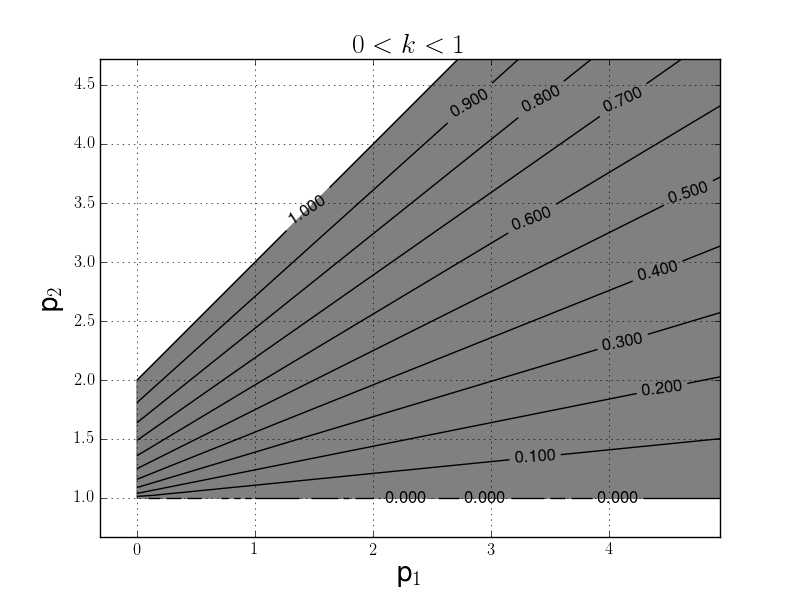
\includegraphics[width = 0.7\linewidth]{Articulated/figure_1.png}
  \caption{Область решения неравенства \ref{articulated:k_condition} для первой конфигурации. Для $k_\tau$ как функции от $p_1$ и $p_2$ линиями показаны уровни значений}
  \label{articulated:fig:case1_dimless_solution}
\end{figure}

Из рисунка \ref{articulated:fig:case1_dimless_solution} можно вывести следующие рекомендации по выбору параметров $h,l$ и $y_c$ с целью снижения необходимого значения $k_\tau$, а именно:

\begin{itemize}
  \item сдвигать центр масс $y_c$ ближе к задним ногам
  \item увеличивать высоту $h$ установки передних ног на вертикальной стенке
  \item уменьшать расстояние $l$ между задними ногами и вертикальной стенкой
\end{itemize}

Перечисленные выше рекомендации используются внутри системы управления робота при планировании следовых точек и при выполнении маневров. Рассмотрим следующую конфигурацию.



\subsection{Вторая конфигурация}
\label{articulated:case_2}

Рассмотрим конфигурацию, когда аппарат опирается на верхнюю горизонтальную и вертикальную площадку.

\begin{figure}[ht]
  \centering
  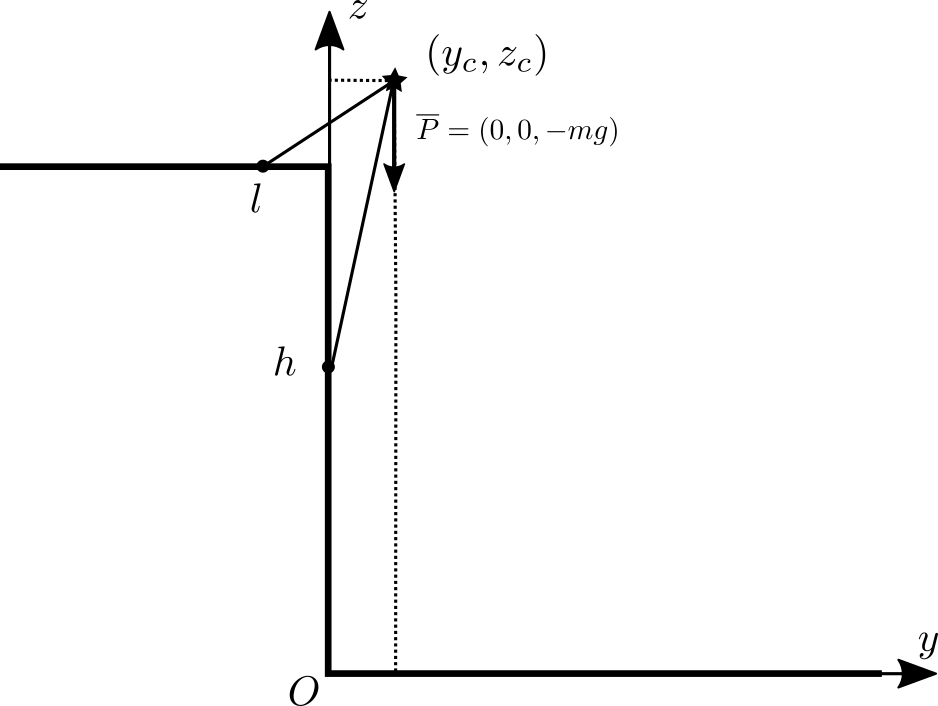
\includegraphics[width=0.7\linewidth]{Articulated/configuration_2.eps}
  \caption{Робот зацепился за верхнюю горизонтальную площадку и опирается на вертикальную площадку}
\end{figure}

Пусть теперь опорные точки ног имею координаты:

\begin{equation}
\label{articulated:case2_step_points}
\begin{alignedat}{3}
&\overline{r}_1 &= (d, l, H) , &\overline{r}_2 &= (-d, l, H) \\
&\overline{r}_3 &= (d, 0, h) , &\overline{r}_4 &= (-d, 0, h) \\
\end{alignedat}, \text{где $l < 0$ и $H > h$ и $l < y_c$.}
\end{equation}

По аналогии с \ref{articulated:case_1_orts} значения ортов $\overline{\tau}_i$, $\overline{\nu}_i$ и $\overline{n}_i$ для рассматриваемой конфигурации имеют вид:

\begin{equation}
\label{articulated:case_2_orts}
\begin{alignedat}{3}
  \overline{\tau}_1 = (0,1,0),&\overline{\nu}_1 = (1,0,0),&\overline{n}_1 = (0,0,1),\\
  \overline{\tau}_2 = (0,1,0),&\overline{\nu}_2 = (1,0,0),&\overline{n}_2 = (0,0,1),\\
  \overline{\tau}_3 = (0,0,1),&\overline{\nu}_3 = (1,0,0),&\overline{n}_3 = (0,1,0),\\
  \overline{\tau}_4 = (0,0,1),&\overline{\nu}_4 = (1,0,0),&\overline{n}_4 = (0,1,0),\\
\end{alignedat}
\end{equation}

Положение центра масс аппарата:

\begin{equation}
\label{articulated:case_2_center_of_gravity}
  \overline{r}_c = (0, y_c, z_c), l < 0, l < y_c,  \text{причем }y_c\text{ может менять свой знак.}
\end{equation}

Выпишем уравнения статики \ref{eq:general_static_equations} для рассматриваемой конфигурации с опорными точками \ref{articulated:case2_step_points} и ортами \ref{articulated:case_2_orts}:

\begin{equation}
  \label{articulated:case2_initial}
\left\{
  \begin{alignedat}{3}
    F_\nu^1 + F_\nu^2 + F_\nu^3 + F_\nu^4 = 0,\\
    F_\tau^1 + F_\tau^2 + N_3 + N_4 = 0,\\
    F_\tau^3 + F_\tau^4 + N_1 + N_2 = P,\\
    N_3 h + N_4 h + P y_c + F_\tau^1 H + F_\tau^2 H = l (N_1 + N_2),\\
    d (F_\tau^3 + N_1) = F_\tau^4 d + F_\nu^3 h + F_\nu^4 h + N_2 d + F_\nu^1 H + F_\nu^2 H,\\
    d (F_\tau^1 + N_3) = F_\tau^2 d + N_4 d + F_\nu^1 l + F_\nu^2 l.\\
  \end{alignedat}
\right.
\end{equation}

 Применим модель кулоновского трения и допущения в симметриях сил трения и распределения нагрузок на ноги робота, в точности как в разделе \ref{articulated:case1} для первой конфигурации. В итоге получим следующую систему из трех  уравнений и тремя неизвестными:

\begin{equation}
\label{eq:case2_final_equations}
\left\{
\begin{alignedat}{3}
  N_d - N_uk_\tau &= 0,\\
  2N_u + 2N_d k_\tau &= P,\\
  2 N_d h + P y_c &= 2 N_u (l + H k_\tau)\\
  \end{alignedat}
\right.
\end{equation}


Из системы \ref{eq:case2_final_equations} находим выражение для  $k_\tau$ при всех $y_c \ne 0$. Возможны два решения:

\begin{equation}
\label{eq:case2_k12}
%      k = 
%      /                2            2        2             \
%      |  H - h + sqrt(H  - 2 H h + h  - 4 y_c  + 4 l y_c)  |
%      |  ------------------------------------------------  |
%      |                        2 y_c                       |
%      |                                                    |
%      |                 2            2        2            |
%      |   h - H + sqrt(H  - 2 H h + h  - 4 y_c  + 4 l y_c) |
%      | - ------------------------------------------------ |
%      \                         2 y_c                      /    
      k_\tau = \dfrac{(H-h) \pm \sqrt{(H-h)^2 - 4y^2_c + 4ly_c}}{2y_c}, \\
\end{equation}

При условиях \ref{articulated:case2_step_points} и \ref{articulated:case_2_orts} рассматриваемой конфигурации, условию $k>0$ из \ref{articulated:k_condition} удовлетворяет только следующее решение:

\begin{equation}
\label{articulated:case2_k_solution}
k_\tau = \dfrac{(H-h) - \sqrt{(H-h)^2 - 4y_c^2 + 4ly_c}}{2y_c}
\end{equation}

Определим при каких параметрах $H,h,l$ и $y_c$ выражение \ref{articulated:case2_k_solution} будет меньше единицы:

\begin{equation}
\label{articulated:case2_k_less_than_1}
\begin{alignedat}{3}
 \dfrac{(H - h) - \sqrt{(H-h)^2 - 4y_c^2+4ly_c}}{2y_c}  & \leq 1 \\
\end{alignedat}
\end{equation}

Введем следующие безразмерные параметры:

\begin{equation}
\label{articulated:case2_dimentionless}
\begin{alignedat}{1}
  p_1 := \dfrac{(H-h)}{y_c}\\
  p_2 := \dfrac{l}{y_c}\\
\end{alignedat}, \text{ где } y_c \ne 0.
\end{equation}

После решения неравенства \ref{articulated:case2_k_less_than_1} и подстановки замены \ref{articulated:case2_dimentionless} в неравенство \ref{articulated:case2_k_less_than_1} получаем следующее решение:


\begin{equation}
\label{articulated:case2_dimless_solution}
\left[
  \begin{alignedat}{1}
    \left\{
      \begin{alignedat}{2}
        p_2 &> 2-p_1,\\
        p_2 &< 0,\\
      \end{alignedat}
    \right.\\
    \left\{
      \begin{alignedat}{2}
        p_2 &< 2- p_1,\\
        p_2 &> 1.\\
      \end{alignedat}
    \right.
  \end{alignedat}
\right.
\end{equation}

Решение \ref{articulated:case2_dimless_solution} изображено на рисунках \ref{articulated:fig:case2_dimless_solution_1} и \ref{articulated:fig:case2_dimless_solution_2}. Так же на рисунках указаны линии уровня для $k_\tau$ как функции от $p_1$ и $p_2$.

\begin{figure}[ht]
  \centering
  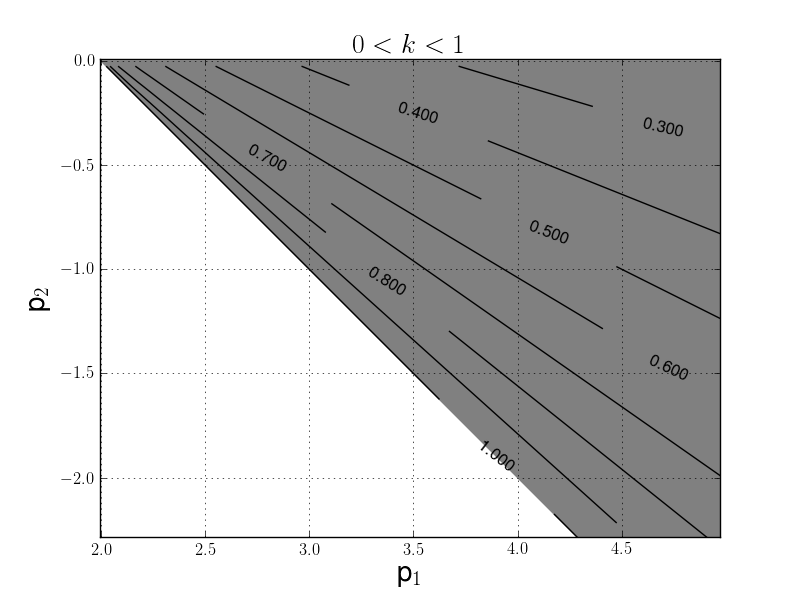
\includegraphics[width = 0.7\linewidth]{Articulated/figure_2_1.png}
  \caption{Область решения неравенства \ref{articulated:k_condition} для второй конфигурации в случае $y_c > 0$. Сплошными линиями показаны уровни значений $k_\tau$.}
  \label{articulated:fig:case2_dimless_solution_1}
\end{figure}

Из рисунка \ref{articulated:fig:case2_dimless_solution_1} можно вывести следующие рекомендации по выбору параметров $h,l$ и $y_c$ для случая $y_c > 0$:

\begin{itemize}
  \item отодвигать центр масс $y_c$ по горизонтали от точки контакта передних ног $l$ с верхней площадкой
  \item уменьшать высоту опоры $h$ задних ног на вертикальную площадку
  \item пододвигать точку опоры $l$ передних ног ближе к краю уступа
\end{itemize}

\begin{figure}[ht]
  \centering
  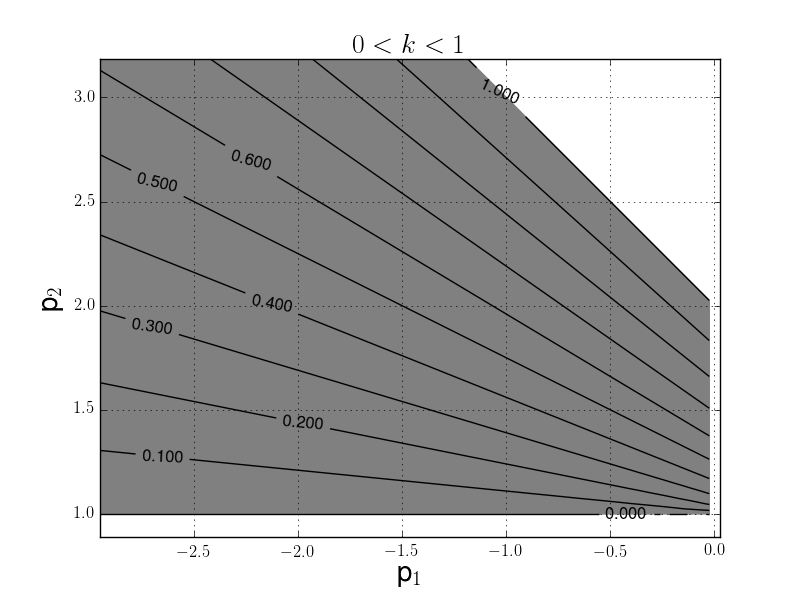
\includegraphics[width=0.7\linewidth]{Articulated/figure_2_2.png}
  \caption{Область решения неравенства \ref{articulated:k_condition} для второй конфигурации в случае $y_c < 0$. Сплошными линиями показаны уровни значений $k_\tau$.}
  \label{articulated:fig:case2_dimless_solution_2}
\end{figure}

Из рисунка \ref{articulated:fig:case2_dimless_solution_2} можно вывести следующие рекомендации по выбору параметров $h,l$ и $y_c$ для случая $y_c < 0$:

\begin{itemize}
  \item сдвигать центр масс $y_c$ в горизонтальной плоскости к точке контакта передних ног
  \item уменьшать высоту опоры $h$ задних ног на вертикальную площадку
  \item пододвигать точку опоры $l$ передних ног ближе к краю уступа
\end{itemize}

Отдельно рассмотрим случай когда центр масс аппарата находится ровно над верхней кромкой уступа.

\subsection{Случай $y_c = 0$}

Подставим $y_c = 0$ в уравнения \ref{eq:case2_final_equations}. Получим:

\begin{equation}
\label{articulated:case2_zero_yc}
\left\{
\begin{alignedat}{3}
N_d - N_uk_\tau &= 0 \\
2N_u+2N_dk_\tau &= P \\
N_dh - N_ul &= HN_uk_\tau\\
\end{alignedat}
\right.
\end{equation}

Из системы \ref{articulated:case2_zero_yc} однозначно получаем:

\begin{equation}
\label{articulated:case2_zero_yc_solution}
\left\{
\begin{alignedat}{3}
&k_\tau = -\dfrac{l}{H-h},\\
&N_u = \dfrac{P(H-h)^2}{2((H-h)^2+l^2)}\\
&N_d = \dfrac{-Pl(H - h)}{2((H-h)^2+l^2)}\\
\end{alignedat}
\right.
\end{equation}

Из условия \ref{articulated:case2_step_points} и \ref{articulated:case2_zero_yc_solution} следует что $k_\tau$ всегда больше нуля. А условие $k_\tau < 1$ будет выполняться когда выполнено следующее соотношение:

\begin{equation}
\label{articulated:case2_zero_yc_simple}
  0 < -l < (H-h)
\end{equation}

Соотношение \ref{articulated:case2_zero_yc_simple} требует что расстояние от передних ног до верхнего края уступа будет меньше, чем расстояние от задних ног до верхнего края уступа.

Таким образом, задача о проверке статической устойчивости шестиногого аппарата свелась к системе из трех уравнений с тремя неизвестными. Рассмотренные конфигурации покрывают все случа расстановки ног, за исключением тривиальных конфигураций, когда выполняется смена опорных ног или когда аппарат опирается ногами только на горизонтальные площадки.

\subsection{Маневры для залезания на уступ}

Робот должен, находясь в начальный момент времени на нижней горизонтальной площадке, подойти к вертикальной стенке уступа и опереться на вертикальную стенку передними ногами. Далее он должен выполняя перестановку ног и артикулируя корпусом дотянуться передними ногами до верхнего края уступа и повиснуть на нём. Затем выполнить перестановку ног и зацепится за верхний край средними ногами, а передние переставить дальше на верхнюю контактную площадку. Затем, выполняется перенос центра масс робота через верхний край уступа и задние ноги переносятся с вертикальной стенки на горизонтальную площадку.

Таким образом, алгоритм залезания робота делится на несколько этапов. Для этапа с номером $n$ введем моменты времени $t_{n-1}$ и $t_n$ --- соответственно моменты начала и конца этапа.

В начальный момент времени $t_0$ корпус ориентирован вдоль оси $Oy$ в положительном направлении. Положение центра $(x,y,z)$ и углы ориентации $(\phi,\psi,\theta)$ для среднего звена корпуса равны:

\begin{equation}
  \begin{alignedat}{2}
    (x,y,z) = (0,0,0.3),\\
    (\phi,\psi,\theta) = (0,0,0)\\
  \end{alignedat}
\end{equation}


Этап 1. Робот переносит передние ноги на вертикальную стенку. Смещает центр масс в сторону стенки и артикулирует передним звеном корпуса. Последовательно переставляет средние и задние ноги ближе к стенке.

Этап 2. Робот переставляет передние ноги еще выше на стенку, остальные ноги переставляются ближе к стенке. Артикулирует всеми звеньями чтобы ноги доставали до точек контакта.

Этап 3. Средние ноги переносятся на вертикальную стенку. Корпус поднимается к верхнему краю уступа. Передние ноги ставятся на верхнюю площадку. Центр масс робота смещается ближе к вертикальной стенке.

Этап 4. Задние ноги поднимаются с нижней площадки и переносятся на вертикальную стенку. Средние ноги переставляются на верхнюю площадку.

Этап 5. Центр масс робота переносится на верхнюю площадку между передними и средними ногами.

Этап 6. Задние ноги переносятся на верхнюю площадку.





\subsubsection{Фаза t1 < t < t2 ...}



